\documentclass{beamer}
\usepackage{animate}
\usepackage{amsmath}
\usepackage{tikz}
\usetheme{Madrid}
\usepackage{tikz}
\usepackage{soul}
\usepackage[normalem]{ulem}
\graphicspath{{./figures/}}

\useinnertheme{circles}
%Information to be included in the title page:
\title{Estimating Relative Changes in RNA Kinetic Rates: What Is It Good For?}
\author{Jakub Koubele}
\institute{Progress Report}
\date{2nd June, 2026}

\renewcommand{\insertshortauthor}{Jakub Koubele}  
\renewcommand{\insertshorttitle}{RNA metabolism kinectics}
\renewcommand{\insertshortdate}{2nd June, 2026} % Define custom text for 3rd block

\usepackage{amsthm}
\newcommand*{\QED}{\hfill\ensuremath{\blacksquare}}


\begin{document}
	\frame{\titlepage}
	
	
\begin{frame}
	\frametitle{Introduction}	
	\pause		
	
	\begin{itemize}			
		
		\item I developed a computational method that estimates difference between LFCs of two different kinetic rates in RNA metabolism, using total RNA-seq. \pause
		\item Now, I am trying to figure out what it is good for.	
		
	\end{itemize}		
		
\end{frame}

\begin{frame}
	\frametitle{RNA metabolism}
	\pause
	\begin{center}
		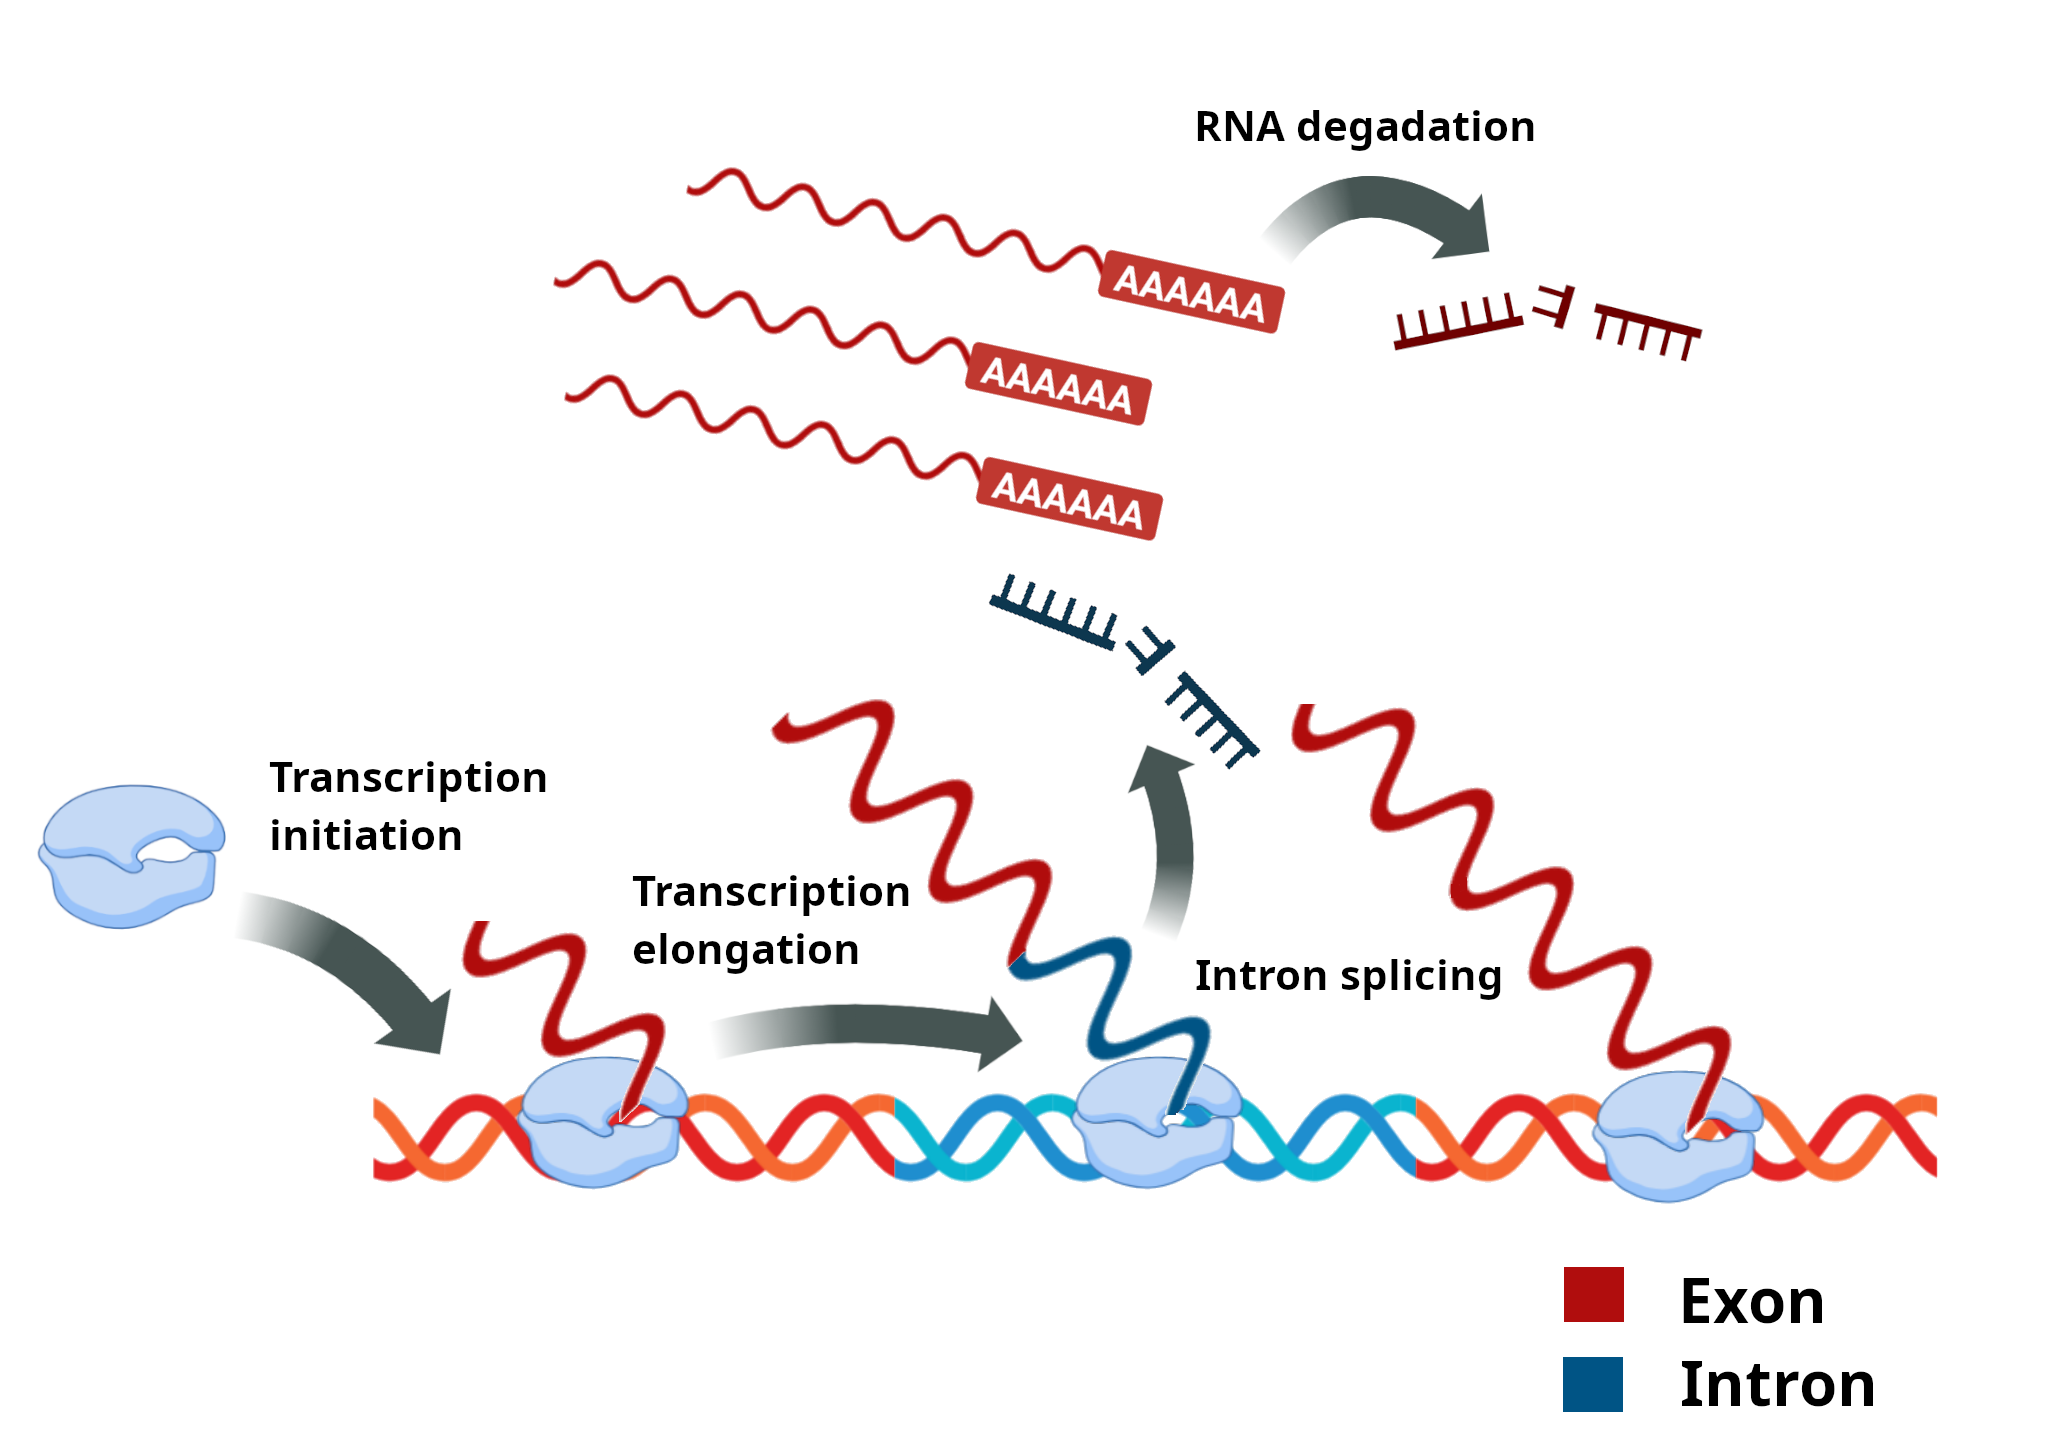
\includegraphics[width=11cm]{rna_metabolism.png}
	\end{center}
	
\end{frame}

\begin{frame}
	\frametitle{Kinetic rates and non-identifability}	
	\begin{itemize}
		\pause
		\item Absolute rates, e.g. $k_{\mathrm{elong}}$, cannot be estimated from total RNA-seq. \pause
		\item Relative rates, e.g. $\mathrm{LFC}(k_{\mathrm{elong}})$, also \textbf{cannot} be estimated from total RNA-seq. \pause
		\item Only changes in ratio of different kinetic rates, e.g. $\mathrm{LFC} \left( \frac{k_{\mathrm{elong}}}{k_{\mathrm{deg}}} \right)$, can be estimated from the data.		
		\pause
		\item This is equivalent to differences in LFCs. 
		E.g., we may estimate the value of 
		$$
		\mathrm{LFC}(k_{\mathrm{elong}}) - \mathrm{LFC}(k_{\mathrm{deg}})
		$$
		and test the hypothesis
		$$
		\mathrm{H}_{0}: \quad \mathrm{LFC}(k_{\mathrm{elong}}) - \mathrm{LFC}(k_{\mathrm{deg}}) = 0
		$$
	\end{itemize}
\end{frame}

\begin{frame}
	\frametitle{Example results: aging mouse myocardium}	
	\pause
	\begin{itemize}
		\item Public dataset \textit{Genomic instability in the naturally and prematurely aged myocardium} (GSE124005).
		\pause
		\item Total RNA samples at 12, 52 and 104 weeks.
				
		$\to$ Between-group comparisons (estimating LFCs of ratios).
		\pause 
		\item My implementation estimates LFCs at different levels of granularity: 
		\begin{itemize}
			\item Whole genome (1 shared LFC vector)
			\item Gene-specific (1 LFC vector per gene)
			\item Intron-specific (1 LFC vector per intron)
		\end{itemize}
	
	$\to$ Trade off - granularity vs. statistical power and robustness.
		
	\end{itemize}
\end{frame}

\begin{frame}
	\frametitle{Aging mouse myocardium: LFC(elongation~speed)~-~LFC(degradation)}
	
	\begin{center}
		\includegraphics[width=12cm]{./aging_mouse_myocardium/lfc_elongation_minus_degradation.png}
	\end{center}
	
\end{frame}

	
\begin{frame}
	\frametitle{Aging mouse myocardium: LFC(splicing~speed)~-~LFC(degradation)}
	
	\begin{center}
		\includegraphics[width=12cm]{./aging_mouse_myocardium/lfc_splicing_minus_degradation.png}
	\end{center}
	
\end{frame}

\begin{frame}
	\frametitle{Aging mouse myocardium: LFC(elongation~speed)~-~LFC(splicing~speed)}
	
	\begin{center}
		\includegraphics[width=12cm]{./aging_mouse_myocardium/lfc_elongation_minus_splicing.png}
	\end{center}
	
\end{frame}

\begin{frame}
	\frametitle{Gene-specific estimates: LFC(elongation~speed)~-~LFC(degradation)}
	
	\begin{center}
		\includegraphics[width=9cm]{./aging_mouse_myocardium/lfc_elongation_minus_degradation_group_wt_104_weeks_vs_wt_12_weeks_gene.png}
	\end{center}
	
\end{frame}

\begin{frame}
	\frametitle{Intron-specific estimates: LFC(elongation~speed)~-~LFC(splicing~speed)}
	
	\begin{center}
		\includegraphics[width=9cm]{./aging_mouse_myocardium/lfc_elongation_minus_splicing_group_wt_104_weeks_vs_wt_12_weeks_intron.png}
	\end{center}
	
\end{frame}

\begin{frame}
	\frametitle{Example results: ENCODE protein KDs}	
	\pause
	\begin{itemize}
		\item Public dataset \textit{Protein knockdown using the auxin-inducible degron} (from the ENCODE project).
		
		\begin{center}
			\includegraphics[width=8cm]{encode.png}
		\end{center}
		
		
	\end{itemize}
\end{frame}

\begin{frame}
	\frametitle{SUPT16H protein knockdown: LFC(elongation~speed)~-~LFC(degradation)}
	
	\begin{center}
		\includegraphics[width=12cm]{encode_degron/lfc_elongation_minus_degradation.png}
	\end{center}

\end{frame}	

\begin{frame}
	\frametitle{SUPT16H protein knockdown: LFC(splicing~speed)~-~LFC(degradation)}
	
	\begin{center}
		\includegraphics[width=12cm]{encode_degron/lfc_splicing_minus_degradation.png}
	\end{center}
	
\end{frame}	

\begin{frame}
	\frametitle{SUPT16H protein knockdown: LFC(elongation~speed)~-~LFC(splicing~speed)}
	
	\begin{center}
		\includegraphics[width=12cm]{encode_degron/lfc_elongation_minus_splicing.png}
	\end{center}
	
\end{frame}	

\begin{frame}
	\frametitle{SUPT16H protein knockdown: intron meta-coverages}
	
	\begin{center}
		\begin{tabular}{cc}
			\includegraphics[width=5.5cm]{encode_degron/all_introns_control.png} &
			\includegraphics[width=5.5cm]{encode_degron/all_introns_degron.png} \\
			Control & Degron
		\end{tabular}
	\end{center}
	
\end{frame}


\begin{frame}
	\frametitle{The End}
	Thank you for your attention!
	
	\begin{center}
		
\includegraphics[width=9cm]{group_picture.jpg}		
	\end{center}	
	
\end{frame}

	
	
\end{document}

